%% ----------------------------------------------------------------------------
%%  §10.2  L'algebra degli o piccoli e il calcolo dei limiti
%% ----------------------------------------------------------------------------
\section{L'algebra degli o piccoli e il calcolo dei limiti}
\label{sec:o-piccoli}

La formula di Taylor con il resto di Peano è lo strumento più efficace per il calcolo
dei limiti che si presentano in forma indeterminata. Cominciamo con un esempio, che ci
mostrerà di quali regole di calcolo abbiamo bisogno.

\begin{esempio}\label{es:limite-taylor-1}
Calcoliamo
\begin{equation}\label{eq:limite-taylor-1}
  \lim_{x\to0}\Bigl(\frac1{x^{2}}-\frac1{x\sen x}\Bigr) ,
\end{equation}
che si presenta nella forma indeterminata $+\infty-(+\infty)$. Riducendo allo stesso
denominatore e usando lo sviluppo $\sen x=x-\frac{x^{3}}6+o(x^{4})$ (la \eqref{eq:taylor-sen} con
$n=1$),
\[
  \frac1{x^{2}}-\frac1{x\sen x}=\frac{\sen x-x}{x^{2}\sen x}
  =\frac{-\frac{x^{3}}6+o(x^{4})}{x^{3}-\frac{x^{5}}6+o(x^{6})} ,
\]
dove abbiamo usato il fatto che $x^{2}\cdot o(x^{4})=o(x^{6})$. Dividendo numeratore e
denominatore per $x^{3}$, e osservando che $\frac{o(x^{4})}{x^{3}}=x\cdot\frac{o(x^{4})}{x^{4}}\to0$ e che
$\frac{o(x^{6})}{x^{3}}\to0$, si ottiene
\[
  \lim_{x\to0}\frac{-\frac16+\frac{o(x^{4})}{x^{3}}}{1-\frac{x^{2}}6+\frac{o(x^{6})}{x^{3}}}=-\frac16 .
\]
Si noti la scelta dell'ordine dello sviluppo. Con il solo $\sen x=x+o(x^{2})$ il numeratore
sarebbe stato $o(x^{2})$, e il rapporto $\frac{o(x^{2})}{x^{3}}$ è ancora indeterminato: occorre
spingere lo sviluppo fino al primo termine che \emph{non si elide}.
\end{esempio}

Nel calcolo precedente abbiamo trattato il simbolo $o(\cdot)$ come se fosse un numero,
sommandolo, moltiplicandolo per potenze, dividendolo. Occorre dare un senso preciso a
queste operazioni.

\begin{notazione}[Uguaglianze con gli o piccoli]
In una formula, il simbolo $o(x^{n})$ (per $x\to0$) indica \emph{una qualsiasi} funzione $f$
tale che $\frac{f(x)}{x^{n}}\to0$; per $n=0$, $o(1)$ indica una qualsiasi funzione infinitesima.
Un'uguaglianza tra espressioni che contengono simboli $o$, come $x^{2}\cdot o(x^{4})=o(x^{6})$,
significa: \emph{ogni} funzione della forma scritta a sinistra è anche della forma
scritta a destra. Queste uguaglianze vanno quindi lette da sinistra a destra, e non sono
simmetriche: $o(x^{2})=o(x)$ è vera (ogni funzione che è $o(x^{2})$ è anche $o(x)$), mentre
$o(x)=o(x^{2})$ è falsa (si pensi a $x^{3/2}$, per $x>0$).
\end{notazione}

\begin{proposizione}[Algebra degli o piccoli]\label{prop:algebra-o}
Per $x\to0$ e per ogni coppia di interi $m,n\ge0$ valgono le proprietà
\begin{align}
  & o(x^{n})+o(x^{n})=o(x^{n}), \qquad o(x^{n})-o(x^{n})=o(x^{n}); \label{eq:o-somma}\\
  & c\cdot o(x^{n})=o(x^{n}), \qquad o(c\,x^{n})=o(x^{n}) \qquad (c\neq0 \text{ costante}); \label{eq:o-costante}\\
  & x^{m}\cdot o(x^{n})=o(x^{m+n}); \label{eq:o-potenza}\\
  & o(x^{m})\cdot o(x^{n})=o(x^{m+n}); \label{eq:o-prodotto}\\
  & o(x^{m})=o(x^{n}) \ \text{ se } m\ge n, \qquad x^{m}=o(x^{n}) \ \text{ se } m>n; \label{eq:o-ordine}\\
  & \frac{o(x^{n})}{x^{m}}=o(x^{n-m}) \qquad (m\le n); \label{eq:o-quoziente}\\
  & o\bigl(o(x^{n})\bigr)=o(x^{n}); \label{eq:o-o}\\
  & o\bigl(x^{n}+o(x^{n})\bigr)=o(x^{n}). \label{eq:o-somma-interna}
\end{align}
\end{proposizione}

\begin{schema}
\Ipotesi{$x\to0$; \ $m,n\ge0$ interi; \ ogni simbolo $o(g)$ denota una funzione $f$ con
$\frac fg\to0$.}
\Tesi{ogni funzione della forma a primo membro delle
\eqref{eq:o-somma}--\eqref{eq:o-somma-interna} è anche della forma a secondo membro.}
\end{schema}

\begin{strategia}
Ogni proprietà si traduce in un'affermazione sui limiti: si scrivono esplicitamente le
funzioni che compaiono a primo membro, si divide per la potenza che compare a secondo
membro e si riconosce, con un'opportuna moltiplicazione e divisione, un prodotto o una
somma di quozienti che tendono a zero per ipotesi. Le ultime due proprietà, in cui un o
piccolo compare \emph{dentro} un altro, richiedono di passare attraverso la funzione
intermedia.
\end{strategia}

\begin{dimostrazione}
Siano $f$ e $g$ funzioni definite vicino a $0$ (escluso al più $0$).

\eqref{eq:o-somma}: se $\frac{f(x)}{x^{n}}\to0$ e $\frac{g(x)}{x^{n}}\to0$, allora
$\frac{f(x)\pm g(x)}{x^{n}}=\frac{f(x)}{x^{n}}\pm\frac{g(x)}{x^{n}}\to0$.

\eqref{eq:o-costante}: se $\frac{f(x)}{x^{n}}\to0$ allora $\frac{c\,f(x)}{x^{n}}=c\,\frac{f(x)}{x^{n}}\to0$; se invece
$\frac{f(x)}{c\,x^{n}}\to0$, allora $\frac{f(x)}{x^{n}}=c\,\frac{f(x)}{c\,x^{n}}\to0$.

\eqref{eq:o-potenza}: se $\frac{f(x)}{x^{n}}\to0$, allora $\frac{x^{m}f(x)}{x^{m+n}}=\frac{f(x)}{x^{n}}\to0$.

\eqref{eq:o-prodotto}: se $\frac{f(x)}{x^{m}}\to0$ e $\frac{g(x)}{x^{n}}\to0$, allora
$\frac{f(x)g(x)}{x^{m+n}}=\frac{f(x)}{x^{m}}\cdot\frac{g(x)}{x^{n}}\to0$.

\eqref{eq:o-ordine}: se $m\ge n$ e $\frac{f(x)}{x^{m}}\to0$, allora $\frac{f(x)}{x^{n}}=x^{m-n}\,\frac{f(x)}{x^{m}}\to0$,
perché $x^{m-n}$ vale $1$ se $m=n$ e tende a $0$ se $m>n$. Se $m>n$, inoltre,
$\frac{x^{m}}{x^{n}}=x^{m-n}\to0$.

\eqref{eq:o-quoziente}: se $\frac{f(x)}{x^{n}}\to0$, allora $\frac{f(x)/x^{m}}{x^{n-m}}=\frac{f(x)}{x^{n}}\to0$.

\eqref{eq:o-o}: sia $g=o(x^{n})$, con $g(x)\neq0$ per $x\neq0$ (condizione richiesta dalla
\cref{def:o-piccolo} perché abbia senso scrivere $o(g)$), e sia $f=o(g)$. Allora
\[
  \frac{f(x)}{x^{n}}=\frac{f(x)}{g(x)}\cdot\frac{g(x)}{x^{n}}\longrightarrow0\cdot0=0 .
\]

\eqref{eq:o-somma-interna}: sia $g(x)=x^{n}+h(x)$ con $h=o(x^{n})$, e sia $f=o(g)$. Poiché
$\frac{g(x)}{x^{n}}=1+\frac{h(x)}{x^{n}}\to1$, la funzione $g$ è diversa da zero vicino a $0$ (per la
permanenza del segno), e
\[
  \frac{f(x)}{x^{n}}=\frac{f(x)}{g(x)}\cdot\frac{g(x)}{x^{n}}
  =\frac{f(x)}{g(x)}\cdot\Bigl(1+\frac{h(x)}{x^{n}}\Bigr)\longrightarrow0\cdot1=0 . \qedhere
\]
\end{dimostrazione}

\begin{attenzione}
Non è lecito scrivere $o(x^{n})-o(x^{n})=0$: i due simboli denotano, in generale, due funzioni
\emph{diverse}, entrambe trascurabili rispetto a $x^{n}$, e la loro differenza è soltanto
un'altra funzione trascurabile rispetto a $x^{n}$, come afferma la \eqref{eq:o-somma}. Ad
esempio $x^{3}=o(x^{2})$ e $2x^{3}=o(x^{2})$, ma $x^{3}-2x^{3}=-x^{3}\neq0$. Per la stessa ragione un
rapporto come $\frac{o(x^{n})}{o(x^{n})}$ non ha alcun significato preciso: può tendere a qualunque
valore, o non avere limite.
\end{attenzione}

Le proprietà \eqref{eq:o-o} e \eqref{eq:o-somma-interna} si generalizzano a un argomento che
sia un qualunque infinitesimo con parte principale nota; è la forma che useremo più
spesso.

\begin{corollario}[o piccoli di infinitesimi con parte principale]\label{cor:o-composto}
Sia $\varphi(x)=a\,x^{k}+o(x^{k})$ per $x\to0$, con $a\neq0$ e $k\ge1$. Allora, per ogni intero
$m\ge1$,
\begin{equation}\label{eq:o-composto}
  \varphi(x)^{m}=a^{m}x^{km}+o(x^{km}), \qquad o\bigl(\varphi(x)^{m}\bigr)=o(x^{km}) .
\end{equation}
\end{corollario}

\begin{schema}
\Ipotesi{$\frac{\varphi(x)}{x^{k}}\to a\neq0$ per $x\to0$; \ $m\ge1$ intero.}
\Tesi{$\frac{\varphi(x)^{m}}{x^{km}}\to a^{m}$; \ se $\frac{f(x)}{\varphi(x)^{m}}\to0$, allora $\frac{f(x)}{x^{km}}\to0$.}
\end{schema}

\begin{strategia}
Tutto discende dal fatto che il rapporto $\frac{\varphi(x)}{x^{k}}$ tende ad $a\neq0$: la potenza
$m$-esima di questo rapporto tende ad $a^{m}$, il che dà la prima uguaglianza. Per la
seconda si procede come per la \eqref{eq:o-o}, scrivendo $\frac{f}{x^{km}}$ come prodotto di
$\frac{f}{\varphi^{m}}$, che tende a zero, e di $\bigl(\frac{\varphi}{x^{k}}\bigr)^{m}$, che resta limitato;
la permanenza del segno garantisce che $\varphi$ non si annulli vicino a $0$.
\end{strategia}

\begin{dimostrazione}
Per ipotesi $\frac{\varphi(x)}{x^{k}}=a+\frac{o(x^{k})}{x^{k}}\to a$, e quindi
$\frac{\varphi(x)^{m}}{x^{km}}=\bigl(\frac{\varphi(x)}{x^{k}}\bigr)^{m}\to a^{m}$, cioè
$\varphi(x)^{m}-a^{m}x^{km}=o(x^{km})$. In particolare $\varphi(x)\neq0$ vicino a $0$, per la permanenza
del segno. Se poi $f=o(\varphi^{m})$,
\[
  \frac{f(x)}{x^{km}}=\frac{f(x)}{\varphi(x)^{m}}\cdot\Bigl(\frac{\varphi(x)}{x^{k}}\Bigr)^{m}\longrightarrow0\cdot a^{m}=0 .
  \qedhere
\]
\end{dimostrazione}

Con questo corollario sono giustificati i calcoli fatti nel \cref{sec:taylor-peano} per la
funzione $1+\sen(e^{x}-1)$: con $u=e^{x}-1=x+o(x)$, si ha $u^{3}=x^{3}+o(x^{3})$ e
$o(u^{3})=o(x^{3})$.

Gli sviluppi di Taylor permettono di confrontare tra loro gli infinitesimi in modo
preciso. Fissiamo il linguaggio.

\begin{definizione}[Ordine di infinitesimo, parte principale, equivalenza]
\label{def:parte-principale}\index{infinitesimo!ordine di}\index{parte principale}
Sia $f$ definita vicino a $0$ (escluso al più $0$). Se esistono un numero $a\neq0$ e un
intero $p\ge0$ tali che
\[
  f(x)=a\,x^{p}+o(x^{p}) \qquad (x\to0),
\]
cioè $\frac{f(x)}{x^{p}}\to a\neq0$, si dice che $f$ è un \emph{infinitesimo di ordine $p$} (se $p\ge1$)
e che $a\,x^{p}$ è la sua \emph{parte principale}. Due funzioni $f$ e $g$ si dicono
\emph{equivalenti} per $x\to0$, e si scrive $f\sim g$, se $\frac{f(x)}{g(x)}\to1$.
\end{definizione}

Ad esempio $\sen x-x$ è un infinitesimo di ordine $3$ con parte principale $-\frac{x^{3}}6$, e
$1-\cos x\sim\frac{x^{2}}2$. Il numero $a$ e l'esponente $p$, quando esistono, sono univocamente
determinati: se fosse anche $f(x)=b\,x^{q}+o(x^{q})$ con $q\neq p$, ad esempio $q>p$ (l'altro
caso è simmetrico), dividendo per $x^{p}$ si avrebbe $\frac{f(x)}{x^{p}}\to0\neq a$; e se $q=p$,
allora $a=b=\lim\frac{f(x)}{x^{p}}$. Una funzione con una parte
principale è equivalente a essa. La proposizione che segue riassume il metodo con cui la
formula di Taylor si usa nel calcolo dei limiti di rapporti.

\begin{proposizione}[Principio della parte principale]\label{prop:parte-principale}
Siano $f(x)=a\,x^{p}+o(x^{p})$ e $g(x)=b\,x^{q}+o(x^{q})$ per $x\to0$, con $a,b\neq0$ e
$p,q\ge0$ interi. Allora
\begin{equation}\label{eq:parte-principale}
  \frac{f(x)}{g(x)}=\frac ab\,x^{p-q}\bigl(1+o(1)\bigr) ;
\end{equation}
in particolare $\frac{f(x)}{g(x)}\to\frac ab$ se $p=q$, e $\frac{f(x)}{g(x)}\to0$ se $p>q$, mentre se $p<q$ il
rapporto diverge in valore assoluto.
\end{proposizione}

\begin{schema}
\Ipotesi{$\frac{f(x)}{x^{p}}\to a\neq0$, \ $\frac{g(x)}{x^{q}}\to b\neq0$ per $x\to0$.}
\Tesi{$\frac{f(x)}{g(x)}\sim\frac ab\,x^{p-q}$: nel limite di un rapporto si possono sostituire numeratore
e denominatore con le loro parti principali.}
\end{schema}

\begin{strategia}
Si confronta il rapporto $\frac fg$ con il rapporto delle parti principali, cioè si mostra
che il loro quoziente tende a $1$. Dividendo numeratore per $x^{p}$ e denominatore per
$x^{q}$, questo quoziente diventa il prodotto di $\frac{f(x)/x^{p}}{a}$ e di
$\frac{b}{g(x)/x^{q}}$, che tendono entrambi a $1$ per ipotesi. Il comportamento di $x^{p-q}$
decide poi il limite.
\end{strategia}

\begin{dimostrazione}
Per $x\neq0$ vicino a $0$ (dove $g(x)\neq0$, per la permanenza del segno applicata a
$\frac{g(x)}{x^{q}}\to b\neq0$),
\[
  \frac{f(x)}{g(x)}\cdot\frac b{a\,x^{p-q}}=\frac{f(x)/x^{p}}{a}\cdot\frac{b}{g(x)/x^{q}}\longrightarrow\frac aa\cdot\frac bb=1 .
\]
Le affermazioni sul limite seguono perché $x^{p-q}$ vale $1$ se $p=q$, tende a $0$ se $p>q$
e diverge in valore assoluto se $p<q$.
\end{dimostrazione}

Nell'\cref{es:limite-taylor-1}, ad esempio, il numeratore $\sen x-x$ ha parte principale
$-\frac{x^{3}}6$ e il denominatore $x^{2}\sen x$ ha parte principale $x^{3}$: il limite è $-\frac16$, senza
altri calcoli. Il problema si riduce dunque a trovare la parte principale del numeratore
e del denominatore, cioè il primo termine non nullo dei loro sviluppi.

\begin{esempio}\label{es:limite-taylor-2}
Calcoliamo
\[
  \lim_{x\to0}\Bigl(\frac1x-\frac{\cos x}{x^{3}}+\frac{\sen3x}{3x^{4}}\Bigr)
  =\lim_{x\to0}\frac{3x^{3}-3x\cos x+\sen3x}{3x^{4}} .
\]
Il denominatore ha parte principale $3x^{4}$; occorre dunque sviluppare il numeratore
almeno fino all'ordine $4$. Ponendo $3x$ al posto di $x$ nello sviluppo del seno
(\cref{lem:sostituzione-o} e \eqref{eq:o-costante}) si ottiene $\sen3x=3x-\frac92\,x^{3}+o(x^{4})$;
inoltre, per la \eqref{eq:taylor-cos} e la \eqref{eq:o-potenza},
$3x\cos x=3x\bigl(1-\frac{x^{2}}2+o(x^{3})\bigr)=3x-\frac32\,x^{3}+o(x^{4})$. Allora
\[
  3x^{3}-3x\cos x+\sen3x=3x^{3}-3x+\frac32\,x^{3}+3x-\frac92\,x^{3}+o(x^{4})=o(x^{4}) ,
\]
e il limite vale $\lim_{x\to0}\frac{o(x^{4})}{3x^{4}}=0$. Tutti i termini fino all'ordine $4$ si sono
elisi. Spingendo gli sviluppi di un ordine (o di due) si trova la parte principale del
numeratore, $\frac{19}{10}\,x^{5}$, e quindi, per la \cref{prop:parte-principale}, la funzione
tende a zero come $\frac{19}{30}\,x$ (\cref{es:verifica-19-30}).
\end{esempio}

\begin{esempio}\label{es:limite-taylor-3}
Studiamo il limite della successione
\[
  \lim_{n\to+\infty}\Bigl(\cos\frac1n\Bigr)^{-n^{2}} .
\]
Per la definizione di limite di funzione mediante successioni (\cref{def:limite-funzione}),
con $x_{n}=\frac1n\to0$, basta calcolare il limite di funzione
\[
  \lim_{x\to0}(\cos x)^{-1/x^{2}}=\lim_{x\to0}e^{-\frac{\log\cos x}{x^{2}}} ,
\]
che è della forma indeterminata $1^{\infty}$. Dalla \eqref{eq:taylor-cos}, $\cos x=1+u$ con
$u=-\frac{x^{2}}2+o(x^{3})$; dalla \eqref{eq:taylor-log} con $n=1$, $\log(1+u)=u+o(u)$, e per il
\cref{cor:o-composto} (con $a=-\frac12$, $k=2$, $m=1$) $o(u)=o(x^{2})$. Dunque
\[
  \log\cos x=-\frac{x^{2}}2+o(x^{3})+o(x^{2})=-\frac{x^{2}}2+o(x^{2}) ,
\]
e quindi $-\frac{\log\cos x}{x^{2}}\to\frac12$. Per la continuità dell'esponenziale (\cref{teo:continuita-esponenziale}) entrambi i
limiti valgono $e^{1/2}=\sqrt e$.
\end{esempio}

\begin{figure}[htb]
\centering
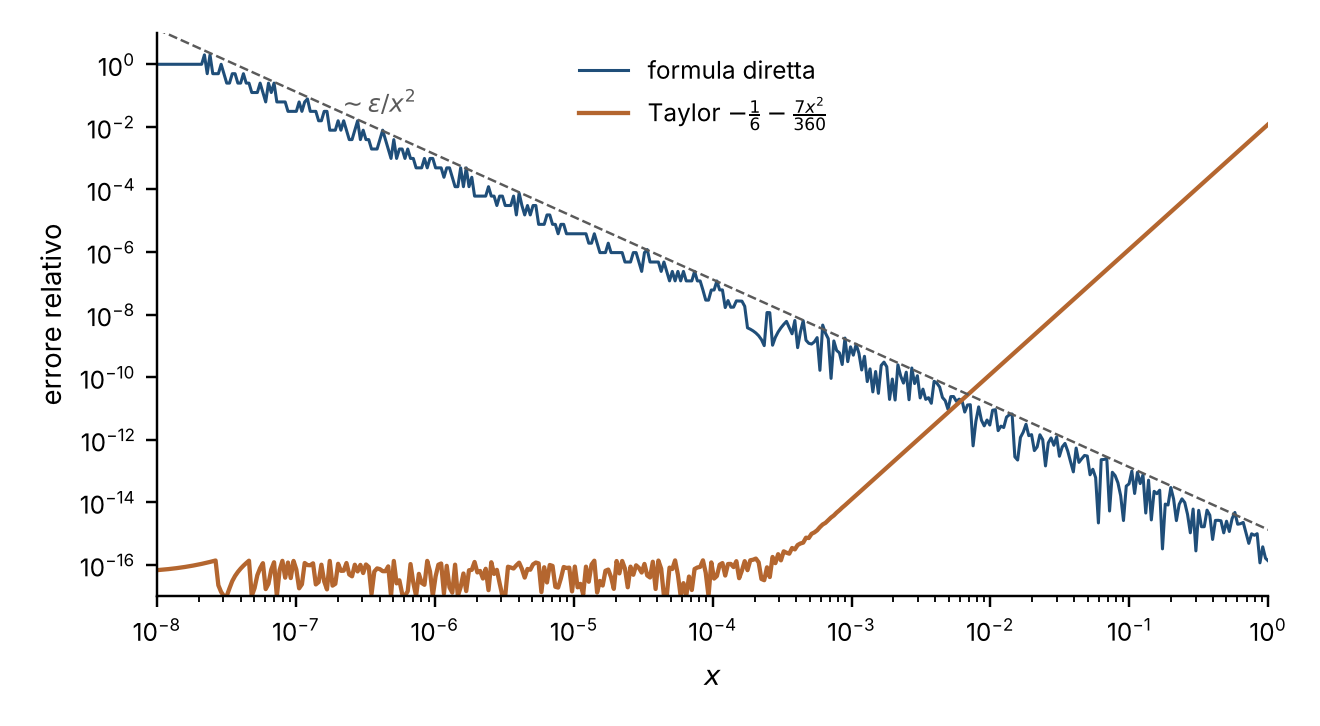
\includegraphics[width=\textwidth]{figure/cancellazione.png}
\caption{Errore relativo nel calcolo di $f(x)=\frac1{x^{2}}-\frac1{x\sen x}$ in aritmetica a
virgola mobile (precisione doppia). La formula diretta (blu) perde cifre come
$\frac{\varepsilon}{x^{2}}$, con $\varepsilon\approx2{,}2\cdot10^{-16}$, per la cancellazione tra due numeri quasi
uguali; il polinomio di Taylor $-\frac16-\frac{7x^{2}}{360}$ (rame) ha un errore che decresce come
$x^{4}$. Le due curve si incrociano per $x$ dell'ordine di $10^{-2}$
(\texttt{python/fig\_cancellazione.py}).}
\label{fig:cancellazione}
\end{figure}

La formula di Taylor non serve soltanto a calcolare limiti «a mano»: è indispensabile
anche nel calcolo numerico. Nel \cref{cap:funzioni-continue} abbiamo incontrato il
fenomeno della \emph{cancellazione}, a proposito di $1-\cos x$ e delle funzioni
\texttt{log1p} ed \texttt{expm1}. La funzione dell'\cref{es:limite-taylor-1}, calcolata con
un computer per $x$ piccolo, ne è un esempio estremo: è la differenza di due numeri
grandi e quasi uguali, ciascuno affetto da un errore di arrotondamento relativo
dell'ordine di $\varepsilon\approx2{,}2\cdot10^{-16}$, e quindi da un errore assoluto dell'ordine di
$\frac\varepsilon{x^{2}}$, che la sottrazione non elimina. Per $x=10^{-8}$ il risultato è privo di
significato. Lo sviluppo $-\frac16-\frac{7x^{2}}{360}+o(x^{3})$ non soffre di questo difetto
(\cref{fig:cancellazione}): la formula di Taylor è il rimedio \emph{sistematico} alla
cancellazione, perché esegue la sottrazione «sulla carta», una volta per tutte. Le
librerie numeriche seguono la stessa idea: per $x$ vicino a zero calcolano funzioni come
\texttt{expm1} e \texttt{log1p} con approssimazioni polinomiali o razionali costruite in
modo da non formare la differenza (i loro coefficienti non sono esattamente quelli di
Taylor, come vedremo nel \cref{sec:tabulazione}), e passano alla formula diretta soltanto
quando la cancellazione non è più pericolosa.

\begin{python}[Limiti con la formula di Taylor: verifica simbolica e numerica]
import math
import sympy as sp
from mpmath import mp, mpf, sin as msin

x = sp.symbols('x')
f = 1 / x**2 - 1 / (x * sp.sin(x))
print(sp.series(f, x, 0, 4))
g = 1 / x - sp.cos(x) / x**3 + sp.sin(3 * x) / (3 * x**4)
print(sp.series(g, x, 0, 3))
print(sp.limit(sp.cos(x)**(-1 / x**2), x, 0))

mp.dps = 40                         # 40 cifre: valore "esatto"
print("     x      formula diretta      Taylor       esatto")
for k in (1, 3, 5, 7, 8):
    t = 10.0**(-k)
    d = 1 / t**2 - 1 / (t * math.sin(t))
    p = -1 / 6 - 7 * t**2 / 360
    e = 1 / mpf(t)**2 - 1 / (mpf(t) * msin(mpf(t)))
    print(f"  1e-{k}  {d:17.12f}  {p:14.12f}  {float(e):14.12f}")
\end{python}
\begin{risultato}
-1/6 - 7*x**2/360 + O(x**4)
19*x/30 + O(x**3)
exp(1/2)
     x      formula diretta      Taylor       esatto
  1e-1    -0.166861316348  -0.166861111111  -0.166861316348
  1e-3    -0.166666686186  -0.166666686111  -0.166666686111
  1e-5    -0.166667938232  -0.166666666669  -0.166666666669
  1e-7    -0.156250000000  -0.166666666667  -0.166666666667
  1e-8     0.000000000000  -0.166666666667  -0.166666666667
\end{risultato}

\begin{notastorica}[I simboli di Landau]
Il simbolo $O$ («o grande»: $f=O(g)$ se $\frac fg$ è limitato) fu introdotto dal teorico dei
numeri tedesco Paul Bachmann nel 1894, nel secondo volume della sua \emph{Zahlentheorie}.
Edmund Landau lo adottò e vi affiancò il simbolo $o$ nel suo trattato sulla distribuzione
dei numeri primi (1909), e da allora entrambi portano il suo nome. L'uso sistematico
degli sviluppi di Taylor per il calcolo dei limiti, però, è molto più antico: già i
matematici del Settecento, a partire da Eulero, trattavano le funzioni come «polinomi
infiniti» e ne confrontavano i termini di grado più basso, anche se senza un controllo
rigoroso del resto. È proprio questo controllo che i simboli di Landau e la formula di
Peano permettono di esercitare con poca fatica.
\end{notastorica}
